\documentclass[10pt,fleqn]{article}
% \usepackage[journal=rsc]{chemstyle}
% \usepackage{mhchem}
\usepackage{amsmath}
\usepackage{amssymb}
\usepackage{amsfonts}
\usepackage{esint}
\usepackage{bbm}
\usepackage{amscd}
\usepackage{picinpar}
\usepackage{graphicx}
\usepackage{tikz}
\usepackage{tikz-3dplot}
\usepackage{indentfirst}
\usepackage{wrapfig}
\usepackage{units}
\usepackage{textcomp}
\usepackage[utf8x]{inputenc}
\usepackage{xkeyval}
\usepackage{xargs}
\usepackage{verbatim}
\usepackage{pgfplots}
\usepackage{hyperref}
\usetikzlibrary{
  arrows,
  calc,
  decorations.pathmorphing,
  decorations.pathreplacing,
  decorations.markings,
  fadings,
  positioning,
  shapes
}

\DeclareGraphicsRule{*}{mps}{*}{}
\newcommand{\ud}{\mathrm{d}}
\newcommand{\ue}{\mathrm{e}}
\newcommand{\ui}{\mathrm{i}}
\newcommand{\res}{\mathrm{Res}}
\newcommand{\Tr}{\mathrm{Tr}}
\newcommand{\dsum}{\displaystyle\sum}
\newcommand{\dprod}{\displaystyle\prod}
\newcommand{\dlim}{\displaystyle\lim}
\newcommand{\dint}{\displaystyle\int}
\newcommand{\fsno}[1]{{\!\not\!{#1}}}
\newcommand{\eqar}[1]
{
  \begin{align*}
    #1
  \end{align*}
}
\newcommand{\texp}[2]{\ensuremath{{#1}\times10^{#2}}}
\newcommand{\dexp}[2]{\ensuremath{{#1}\cdot10^{#2}}}
\newcommand{\eval}[2]{{\left.{#1}\right|_{#2}}}
\newcommand{\paren}[1]{{\left({#1}\right)}}
\newcommand{\lparen}[1]{{\left({#1}\right.}}
\newcommand{\rparen}[1]{{\left.{#1}\right)}}
\newcommand{\abs}[1]{{\left|{#1}\right|}}
\newcommand{\sqr}[1]{{\left[{#1}\right]}}
\newcommand{\crly}[1]{{\left\{{#1}\right\}}}
\newcommand{\angl}[1]{{\left\langle{#1}\right\rangle}}
\newcommand{\tpdiff}[4][{}]{{\paren{\frac{\partial^{#1} {#2}}{\partial {#3}{}^{#1}}}_{#4}}}
\newcommand{\tpsdiff}[4][{}]{{\paren{\frac{\partial^{#1}}{\partial {#3}{}^{#1}}{#2}}_{#4}}}
\newcommand{\pdiff}[3][{}]{{\frac{\partial^{#1} {#2}}{\partial {#3}{}^{#1}}}}
\newcommand{\diff}[3][{}]{{\frac{\ud^{#1} {#2}}{\ud {#3}{}^{#1}}}}
\newcommand{\psdiff}[3][{}]{{\frac{\partial^{#1}}{\partial {#3}{}^{#1}} {#2}}}
\newcommand{\sdiff}[3][{}]{{\frac{\ud^{#1}}{\ud {#3}{}^{#1}} {#2}}}
\newcommand{\tpddiff}[4][{}]{{\left(\dfrac{\partial^{#1} {#2}}{\partial {#3}{}^{#1}}\right)_{#4}}}
\newcommand{\tpsddiff}[4][{}]{{\paren{\dfrac{\partial^{#1}}{\partial {#3}{}^{#1}}{#2}}_{#4}}}
\newcommand{\pddiff}[3][{}]{{\dfrac{\partial^{#1} {#2}}{\partial {#3}{}^{#1}}}}
\newcommand{\ddiff}[3][{}]{{\dfrac{\ud^{#1} {#2}}{\ud {#3}{}^{#1}}}}
\newcommand{\psddiff}[3][{}]{{\frac{\partial^{#1}}{\partial{}^{#1} {#3}} {#2}}}
\newcommand{\sddiff}[3][{}]{{\frac{\ud^{#1}}{\ud {#3}{}^{#1}} {#2}}}
\usepackage{fancyhdr}
\usepackage{multirow}
\usepackage{fontenc}
% \usepackage{tipa}
\usepackage{ulem}
\usepackage{color}
\usepackage{cancel}
\newcommand{\hcancel}[2][black]{\setbox0=\hbox{#2}%
  \rlap{\raisebox{.45\ht0}{\textcolor{#1}{\rule{\wd0}{1pt}}}}#2}
\pagestyle{fancy}
\setlength{\headheight}{67pt}
\fancyhead{}
\fancyfoot{}
\fancyfoot[C]{\thepage}
\fancyhead[R]{}
\renewcommand{\footruleskip}{0pt}
\renewcommand{\headrulewidth}{0.4pt}
\renewcommand{\footrulewidth}{0pt}

\newcommand\pgfmathsinandcos[3]{%
  \pgfmathsetmacro#1{sin(#3)}%
  \pgfmathsetmacro#2{cos(#3)}%
}
\newcommand\LongitudePlane[3][current plane]{%
  \pgfmathsinandcos\sinEl\cosEl{#2} % elevation
  \pgfmathsinandcos\sint\cost{#3} % azimuth
  \tikzset{#1/.estyle={cm={\cost,\sint*\sinEl,0,\cosEl,(0,0)}}}
}
\newcommand\LatitudePlane[3][current plane]{%
  \pgfmathsinandcos\sinEl\cosEl{#2} % elevation
  \pgfmathsinandcos\sint\cost{#3} % latitude
  \pgfmathsetmacro\yshift{\cosEl*\sint}
  \tikzset{#1/.estyle={cm={\cost,0,0,\cost*\sinEl,(0,\yshift)}}} %
}
\newcommand\DrawLongitudeCircle[2][1]{
  \LongitudePlane{\angEl}{#2}
  \tikzset{current plane/.prefix style={scale=#1}}
  % angle of "visibility"
  \pgfmathsetmacro\angVis{atan(sin(#2)*cos(\angEl)/sin(\angEl))} %
  \draw[current plane] (\angVis:1) arc (\angVis:\angVis+180:1);
  \draw[current plane,dashed] (\angVis-180:1) arc (\angVis-180:\angVis:1);
}
\newcommand\DrawLatitudeCircleArrow[2][1]{
  \LatitudePlane{\angEl}{#2}
  \tikzset{current plane/.prefix style={scale=#1}}
  \pgfmathsetmacro\sinVis{sin(#2)/cos(#2)*sin(\angEl)/cos(\angEl)}
  % angle of "visibility"
  \pgfmathsetmacro\angVis{asin(min(1,max(\sinVis,-1)))}
  \draw[current plane,decoration={markings, mark=at position 0.6 with {\arrow{<}}},postaction={decorate},line width=.6mm] (\angVis:1) arc (\angVis:-\angVis-180:1);
  \draw[current plane,dashed,line width=.6mm] (180-\angVis:1) arc (180-\angVis:\angVis:1);
}
\newcommand\DrawLatitudeCircle[2][1]{
  \LatitudePlane{\angEl}{#2}
  \tikzset{current plane/.prefix style={scale=#1}}
  \pgfmathsetmacro\sinVis{sin(#2)/cos(#2)*sin(\angEl)/cos(\angEl)}
  % angle of "visibility"
  \pgfmathsetmacro\angVis{asin(min(1,max(\sinVis,-1)))}
  \draw[current plane] (\angVis:1) arc (\angVis:-\angVis-180:1);
  \draw[current plane,dashed] (180-\angVis:1) arc (180-\angVis:\angVis:1);
}
\newcommand\coil[1]{
  {\rh * cos(\t * pi r)}, {\apart * (2 * #1 + \t) + \rv * sin(\t * pi r)}
}
\makeatletter
\define@key{DrawFromCenter}{style}[{->}]{
  \tikzset{DrawFromCenterPlane/.style={#1}}
}
\define@key{DrawFromCenter}{r}[1]{
  \def\@R{#1}
}
\define@key{DrawFromCenter}{center}[(0, 0)]{
  \def\@Center{#1}
}
\define@key{DrawFromCenter}{theta}[0]{
  \def\@Theta{#1}
}
\define@key{DrawFromCenter}{phi}[0]{
  \def\@Phi{#1}
}
\presetkeys{DrawFromCenter}{style, r, center, theta, phi}{}
\newcommand*\DrawFromCenter[1][]{
  \setkeys{DrawFromCenter}{#1}{
    \pgfmathsinandcos\sint\cost{\@Theta}
    \pgfmathsinandcos\sinp\cosp{\@Phi}
    \pgfmathsinandcos\sinA\cosA{\angEl}
    \pgfmathsetmacro\DX{\@R*\cost*\cosp}
    \pgfmathsetmacro\DY{\@R*(\cost*\sinp*\sinA+\sint*\cosA)}
    \draw[DrawFromCenterPlane] \@Center -- ++(\DX, \DY);
  }
}
\newcommand*\DrawFromCenterText[2][]{
  \setkeys{DrawFromCenter}{#1}{
    \pgfmathsinandcos\sint\cost{\@Theta}
    \pgfmathsinandcos\sinp\cosp{\@Phi}
    \pgfmathsinandcos\sinA\cosA{\angEl}
    \pgfmathsetmacro\DX{\@R*\cost*\cosp}
    \pgfmathsetmacro\DY{\@R*(\cost*\sinp*\sinA+\sint*\cosA)}
    \draw[DrawFromCenterPlane] \@Center -- ++(\DX, \DY) node {#2};
  }
}
\makeatother
\tikzstyle{snakearrow} = [decorate, decoration={pre length=0.2cm,
  post length=0.2cm, snake, amplitude=.4mm,
  segment length=2mm},thick, ->]
%% document-wide tikz options and styles
\tikzset{%
  >=latex, % option for nice arrows
  inner sep=0pt,%
  outer sep=2pt,%
  mark coordinate/.style={inner sep=0pt,outer sep=0pt,minimum size=3pt,
    fill=black,circle}%
}
\addtolength{\hoffset}{-1.3cm}
\addtolength{\voffset}{-2cm}
\addtolength{\textwidth}{3cm}
\addtolength{\textheight}{2.5cm}
\renewcommand{\footskip}{10pt}
\setlength{\headwidth}{\textwidth}
\setlength{\headsep}{20pt}
\setlength{\marginparwidth}{0pt}
\parindent=0pt
\title{Response of single bit rotation to amplitude noise}

\ifpdf
  % Ensure reproducible output
  \pdfinfoomitdate=1
  \pdfsuppressptexinfo=-1
  \pdftrailerid{}
  \hypersetup{
    pdfcreator={},
    pdfproducer={}
  }
\fi

\begin{document}

\maketitle

\section{Goal}
Try to derive the pulse sequence to achieve robustness against (DC) amplitude noise
in a brute force/generic way.

\section{Pulse sequence with three rotations}
\begin{enumerate}
\item $\sigma_1\equiv\sigma_x\cos\theta_1+\sigma_y\sin\theta_1$ by angle $\psi_1$
\item $\sigma_2\equiv\sigma_x$ by angle $\psi_2$
\item $\sigma_3\equiv\sigma_x\cos\theta_3+\sigma_y\sin\theta_3$ by angle $\psi_3$
\end{enumerate}

Full rotation.
\eqar{
  U=&\exp\paren{\ui\psi_1\sigma_1/2}\exp\paren{\ui\psi_2\sigma_2/2}\exp\paren{\ui\psi_3\sigma_3/2}
}

When $\psi_1$, $\psi_2$, $\psi_3$ are changed by a small fraction $2\varepsilon$ to
$\psi_1\paren{1+2\varepsilon}$, $\psi_2\paren{1+2\varepsilon}$,
$\psi_3\paren{1+2\varepsilon}$ respectively.\\

The derivative of $U$ w.r.t. $\varepsilon$ is.
\eqar{
  \pdiff{U}{\varepsilon}=&\ui\psi_1\exp\paren{\ui\psi_1\sigma_1/2}\sigma_1\exp\paren{\ui\psi_2\sigma_2/2}\exp\paren{\ui\psi_3\sigma_3/2}+\\
  &\ui\psi_2\exp\paren{\ui\psi_1\sigma_1/2}\sigma_2\exp\paren{\ui\psi_2\sigma_2/2}\exp\paren{\ui\psi_3\sigma_3/2}+\\
  &\ui\psi_3\exp\paren{\ui\psi_1\sigma_1/2}\exp\paren{\ui\psi_2\sigma_2/2}\sigma_3\exp\paren{\ui\psi_3\sigma_3/2}
}
Simplifying it by changing coordinates
\eqar{
  &\exp\paren{-\ui\psi_1\sigma_1/2}\pdiff{U}{\varepsilon}\exp\paren{-\ui\psi_2\sigma_2/2}\exp\paren{-\ui\psi_3\sigma_3/2}\\
  =&\ui\psi_1\sigma_1+\ui\psi_2\sigma_2+
  \ui\psi_3\exp\paren{\ui\psi_2\sigma_2/2}\sigma_3\exp\paren{-\ui\psi_2\sigma_1/2}\\
  =&\ui\psi_1\sigma_1+\ui\psi_2\sigma_2+
  \ui\psi_3\paren{\sigma_3\cos\psi_2-\sigma_z\sin\theta_3\sin\psi_2+\sigma_2\cos\theta_3(1-\cos\psi_2)}
}
For this to be $0$, the coefficient for $\sigma_z$ has to be $0$.
This means $\psi_3=0$ (two rotation only), $\sin\theta_3=0$
(third rotation on the same axis as the second one, so effectivel no third rotation),
or $\sin\psi_2=0$. For a true three rotation sequence,
the only option is $\sin\psi_2=0$,
which leave us with two possibilities $\cos\psi_2=\pm1$.\\

For $\cos\psi_2=1$,
\eqar{
  &\exp\paren{-\ui\psi_1\sigma_1/2}\pdiff{U}{\varepsilon}\exp\paren{-\ui\psi_2\sigma_2/2}\exp\paren{-\ui\psi_3\sigma_3/2}\\
  =&\ui\psi_1\sigma_1+\ui\psi_2\sigma_2+\ui\psi_3\sigma_3
}

For $\cos\psi_2=-1$,
\eqar{
  &\exp\paren{-\ui\psi_1\sigma_1/2}\pdiff{U}{\varepsilon}\exp\paren{-\ui\psi_2\sigma_2/2}\exp\paren{-\ui\psi_3\sigma_3/2}\\
  =&\ui\psi_1\sigma_1+\ui\psi_2\sigma_2+
  \ui\psi_3\paren{-\sigma_3+2\sigma_2\cos\theta_3}\\
  =&\ui\psi_1\sigma_1+\ui\psi_2\sigma_2+
  \ui\psi_3\paren{\sigma_x\cos\theta_3-\sigma_y\sin\theta_3}
}

For both of these cases, the robust condition is for the sum of
the three Pauli vectors to be $0$
(in the first case these are the Pauli vector that corresponds to the rotation
and in the second case the last one is replaced
with its reflection about the $x$ axis).
The robust condition for the first one
is also the same as the cross talk calculation condition which allows
the pulse sequence to cancel cross talk and overrotation error to the first order
at the same time.\\

As for the actual rotation, for the first case, the second pulse is a full rotation
so the equivalent final operation is simply the combination
of the first and the third one. Unless one of them is a $\pi$ or $2\pi$ rotation,
the combined result will have a component that is a $z$ rotation.
This operation cannot be removed by changing the coordinate system
(i.e. by making the second rotation along another axis rather than the $x$ axis).
This could be cancelled out for single-qubit gate by adjusting the phase
but may not be as easy for two-qubit gates.\\

For the second case,
\eqar{
  U=&\exp\paren{\ui\psi_1\sigma_1/2}\sigma_x\exp\paren{\ui\psi_3\sigma_3/2}\\
  =&\paren{\cos\frac{\psi_1}{2}+\ui\sigma_x\cos\theta_1\sin\frac{\psi_1}{2}+\ui\sigma_y\sin\theta_1\sin\frac{\psi_1}{2}}\sigma_x\paren{\cos\frac{\psi_3}{2}+\ui\sigma_x\cos\theta_3\sin\frac{\psi_3}{2}+\ui\sigma_y\sin\theta_3\sin\frac{\psi_3}{2}}\\
  =&\sigma_x\cos\frac{\psi_1}{2}\cos\frac{\psi_3}{2}+\ui\cos\frac{\psi_1}{2}\cos\theta_3\sin\frac{\psi_3}{2}-\sigma_z\cos\frac{\psi_1}{2}\sin\theta_3\sin\frac{\psi_3}{2}\\
  &+\ui\cos\theta_1\sin\frac{\psi_1}{2}\cos\frac{\psi_3}{2}-\sigma_x\cos\theta_1\cos\theta_3\sin\frac{\psi_1}{2}\sin\frac{\psi_3}{2}-\sigma_y\cos\theta_1\sin\theta_3\sin\frac{\psi_1}{2}\sin\frac{\psi_3}{2}\\
  &+\sigma_z\sin\theta_1\sin\frac{\psi_1}{2}\cos\frac{\psi_3}{2}-\sigma_y\sin\theta_1\cos\theta_3\sin\frac{\psi_1}{2}\sin\frac{\psi_3}{2}+\sigma_x\sin\theta_1\sin\theta_3\sin\frac{\psi_1}{2}\sin\frac{\psi_3}{2}\\
  =&\ui\cos\theta_3\cos\frac{\psi_1}{2}\sin\frac{\psi_3}{2}+\ui\cos\theta_1\sin\frac{\psi_1}{2}\cos\frac{\psi_3}{2}\\
  &+\sigma_x\cos\frac{\psi_1}{2}\cos\frac{\psi_3}{2}-\sigma_x\cos\theta_1\cos\theta_3\sin\frac{\psi_1}{2}\sin\frac{\psi_3}{2}+\sigma_x\sin\theta_1\sin\theta_3\sin\frac{\psi_1}{2}\sin\frac{\psi_3}{2}\\
  &-\sigma_y\cos\theta_1\sin\theta_3\sin\frac{\psi_1}{2}\sin\frac{\psi_3}{2}-\sigma_y\sin\theta_1\cos\theta_3\sin\frac{\psi_1}{2}\sin\frac{\psi_3}{2}\\
  &-\sigma_z\sin\theta_3\cos\frac{\psi_1}{2}\sin\frac{\psi_3}{2}+\sigma_z\sin\theta_1\sin\frac{\psi_1}{2}\cos\frac{\psi_3}{2}
}
(Seems possible to achieve pure $x-y$ plane rotation though not sure if there's a way
to express the condition in a concise way.)

\subsection{Maximizing the final rotation angle}
Given the same total pulse lens (i.e. total rotation angle for all the pulses),
we'd like to maximize the total effective rotation angle to make the pulse sequence
the most efficient.\\

\begin{figure}[h]
  \centering
  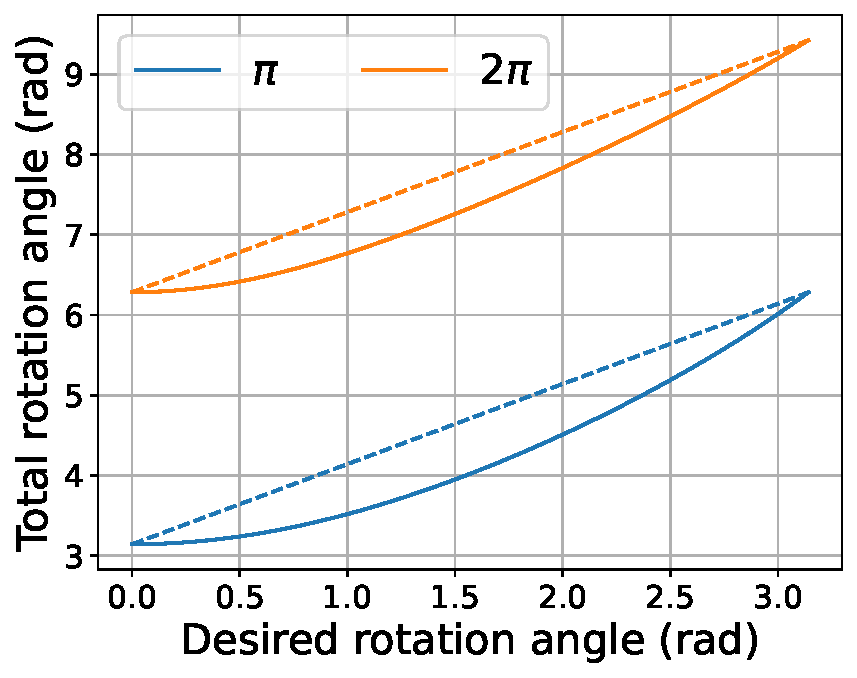
\includegraphics[width=9cm]{imgs/three_pulses.pdf}
  \caption{Minimum angle required to implement a total rotation angle.
    Rotation around $z$ is ignored in the final rotation angle and only rotation
    around an axis in the $xy$ plane is shown.
    The exact axis is also omitted from the plot since it can be changed to any
    desired direction by changing the axis of all the rotations at the same time.
    The legend shows the length of the middle pulse which is chosen to be $\pi$
    for the $\cos\psi_2=-1$ case and $2\pi$ for the $\cos\psi_2=1$.
    The dashed line shows the corresponding total pulse length for the SK1(-like)
    pulse sequence where the first (or the last) pulse
    has the desired rotation angle.}
  \label{fig:three-pulses}
\end{figure}

Fig.~\ref{fig:three-pulses} shows the result of numerically optimizing
the pulse sequnece by computing the maximum achievable rotation angle
for a fixed total rotation angle (time). Two cases that corresponds to
the minimum length second pulse are shown i.e. $\psi_2=\pi$ and $\psi_2=2\pi$.
The dashed line shows the comparison to the corresponding SK1(-like) pulse sequence.
Since the total pulse sequence length must be at least
twice the length of the second pulse, the improvement on top of the SK1 sequence
is not very significant and is at most about $10\%$.

\clearpage
\appendix
\section{Decompose an arbitray single qubit rotation into an $xy$ rotation
  and a $z$ rotation}

Arbitrary single qubit rotation,
\eqar{
  U=&a_0 + x_0 \sigma_x + y_0 \sigma_y + z_0 \sigma_z
}
$xy$ rotation followed by $z$ rotation with global phase
\eqar{
  U=&U_{xy} U_z\ue^{\ui\phi}\\\
  =&\paren{a_1 + x_1 \sigma_x + y_1 \sigma_y}\paren{\cos\theta + \ui\sin\theta\sigma_z}\ue^{\ui\phi}\\
  =&\paren{a_1\cos\theta + \ui a_1\sin\theta \sigma_z + \cos\theta x_1 \sigma_x + \ui\sin\theta x_1 \sigma_x\sigma_z + \cos\theta y_1 \sigma_y + \ui\sin\theta y_1 \sigma_y\sigma_z}\ue^{\ui\phi}\\
  =&\paren{a_1\cos\theta + \paren{\cos\theta x_1 - \sin\theta y_1} \sigma_x + \paren{\cos\theta y_1 + \sin\theta x_1} \sigma_y + \ui a_1\sin\theta \sigma_z}\ue^{\ui\phi}
}
where $a_1$ is a real numbers.
\eqar{
  a_0\ue^{-\ui\phi}=&a_1\cos\theta\\
  x_0\ue^{-\ui\phi}=&x_1\cos\theta - y_1\sin\theta\\
  y_0\ue^{-\ui\phi}=&y_1\cos\theta + x_1\sin\theta\\
  z_0\ue^{-\ui\phi}=&\ui a_1\sin\theta
}

so we have
\eqar{
  a_1=&\sqrt{\abs{a_0}^2+\abs{z_0}^2}\\
  \cos\theta=&\frac{\abs{a_0}}{\sqrt{\abs{a_0}^2+\abs{z_0}^2}}\\
  \sin\theta=&\frac{\abs{z_0}}{\sqrt{\abs{a_0}^2+\abs{z_0}^2}}\\
  x_1=&\frac{a_0^*x_0-\ui z_0y_0^*}{\sqrt{\abs{a_0}^2+\abs{z_0}^2}}\\
  y_1=&\frac{a_0^*y_0+\ui z_0x_0^*}{\sqrt{\abs{a_0}^2+\abs{z_0}^2}}
}

\end{document}
